
\chapter{Rules}

SCHC  works between two entities. Usually, one is a constrained end-device and the other one is a core equipment acting as a router. To allow both of them to perform the same actions, or more precisely one action and a reverse action, such as compression and decompression or fragmentation and reassembly, a common set of rules must be shared between these two entities.

~

The distinction between a device and a core allows to differentiate communication going upstream from the device to the core and downstream in the opposite direction. The device usually owns a limited number of rules corresponding to the traffic  generated and received by that device. On the contrary, the core instance of SCHC must be aware of all the devices' rules. Even if all the devices have the same behavior, SCHC treats each device individually. 

~~

All rules are identified by a \Index{rule ID}. The rule ID is a unique binary sequence for an association between a device and a core. The rule ID length is not specified by the standard and are chosen when the rules are specified. They must be different inside a set of rule. The only constraint is that rule ID cannot overlap.

For instance:

\begin{itemize}
\item\texttt{0} and \texttt{111111} are two valid rules ID
\item \texttt{01} and \texttt{0101} not not valid since they share the same first two bits.
\end{itemize}

~


Rules may be represented in binary, but the decimal notation is also used for compactness. In this book, we will represent a rule ID with the \texttt{rule ID value/rule ID length}. For instance \texttt{3/8} indicates a rule ID stored on 8 bits with value 3.

~

This notation can be misleading, if \texttt{1/2} and \texttt{127/8} taken from the example above are overlapping since they both start with \texttt{01}, \texttt{12/4} and \texttt{12/6} are two valuable rules, since when written in binary \texttt{1100} and \texttt{001100} do not share a common binary sequence.

\begin{figure}[tbp]
\centerline{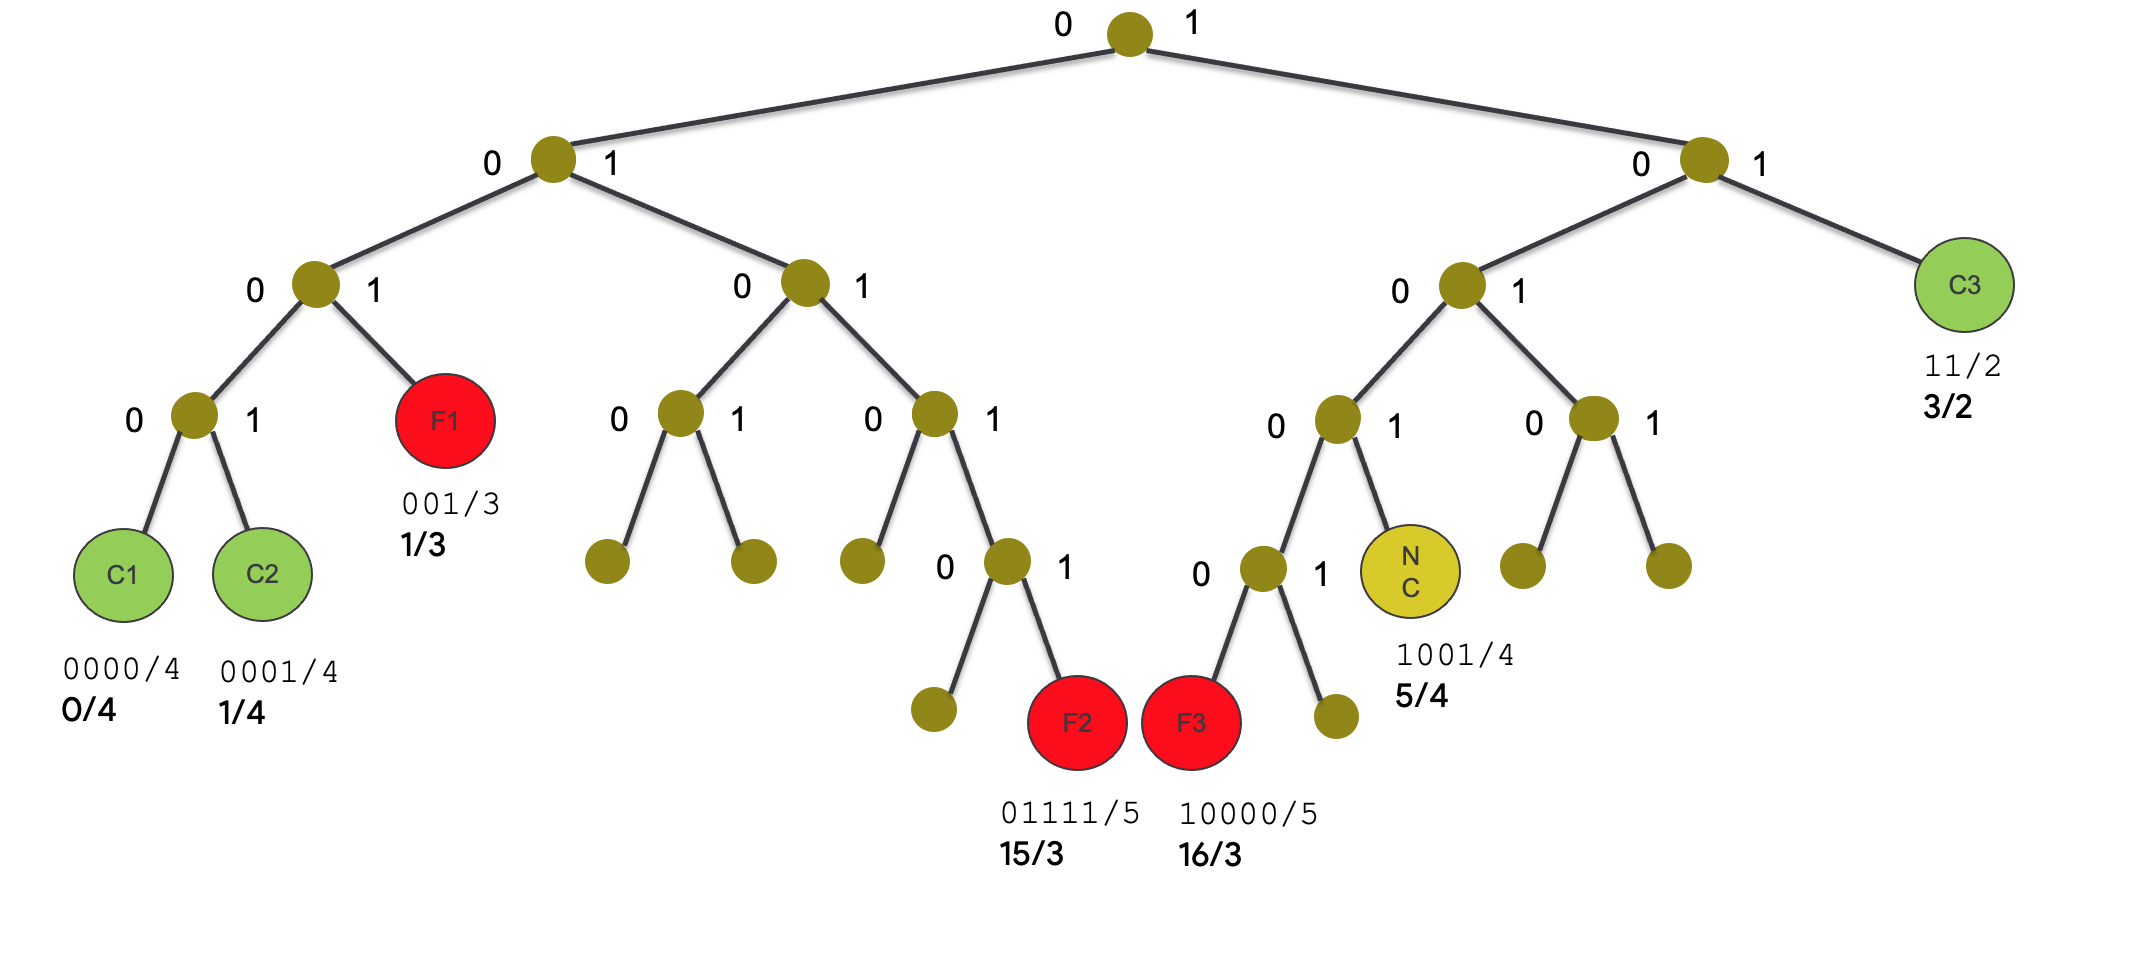
\includegraphics[width=1\columnwidth]{Pictures/binary-rule.png}}
\lge{\caption{Example of binary tree associated to rule IDs}}
\label{fig-base64}
\end{figure}

\section{openSCHC rules}

In openSCHC, a rule is defined in a JSON object:

\begin{lstlisting}[backgroundcolor=\color{yellow}]
    {
    "RuleID" : 12,
    "RuleIDLength" : 4
    }
\end{lstlisting}

There is two different rule formats, one for compression and the other for fragmentation. \Index{Compression} Rules contains the keyword \texttt{Compression} followed by an array, as shown the the minimal example below: 

\begin{lstlisting}[backgroundcolor=\color{yellow}]
   {
   "RuleID" : 12,
   "RuleIDLength" : 4,
   "Compression" : []
   }
   
\end{lstlisting}

   
\Index{Fragmentation} rules uses the \texttt{Fragmentation} keyword followed by an object giving fragmentation parameters:

\begin{lstlisting}[backgroundcolor=\color{yellow}]
    {
    "RuleID" : 12,
    "RuleIDLength" : 6,
    "Fragmentation" : {
      "FRMode" : "NoAck",
      "FRDirection" : "UP"
    }
\end{lstlisting}

Fragmentation and compression rules share the same rule space, by construction a rule cannot be both compression and fragmentation. 
An attentive reader may have also noticed that a fragmentation direction is present in the rule description. 
In fact, compression rules are bi-directionnal and may be used to compress an header by the device and the core, but fragmentation rules are oriented.  

~

Finally a \Index{\texttt{NoCompression}} keyword also exists and is the equivalent to the above example, indicating an uncompressed packet.

\begin{lstlisting}[backgroundcolor=\color{yellow}]
   {
   "RuleID" : 666,
   "RuleIDLength" : 10,
   "NoCompression" : []
   }
\end{lstlisting}


\section{Rule Manager}

The \Index{Rule Manager} plays an important role in openSCHC. It has different goals:
\begin{itemize}
    \item check the rule correctness
    \item add default parameters, to simplify rule notation
    \item display rules in a more synthetic format
    \item find the best rule to compress or fragment a packet
    \item find a rule from its rule ID.
\end{itemize}

\subsection{Rule definition}

The above listing gives a simple python program used to manage the two rules we described before. 

\pythonlst{rm1.py}

This program import the \texttt{gen\_rulemanager} module defining the \texttt{\pfunction{gen\_rulemanager}{RuleManager}} class. 

~~


The \texttt{\pfunction{gen\_rulemanager}{Add}} method allows to add a new rule.

~~~

OpenSCHC displays, with the \pfunction{gen\_rulemanager}{Print}:

\begin{termc}[backgroundcolor=\color{palerod}, basicstyle=\ttfamily\tiny, escapechar=@]
****************************************
Device: None
/-------------------------\
|Rule 12/4          1100  |
|---------------+---+--+--+------------------------------+-------------+----------------\
\---------------+---+--+--+------------------------------+-------------+----------------/
/-------------------------\
|Rule 12/6        001100  |
!=========================+=============================================================\
!^ Fragmentation mode : noAck    header dtag 2 Window  0 FCN  3                     UP ^!
!^ No Tile size specified                                                              ^!
!^ RCS Algorithm: crc32                                                                ^!
\=======================================================================================/
\end{termc}

Compression rules contain the field descriptions (here empty) and Fragmentation rules contain the fragmentation parameters. Note that for fragmentation, the rule manager added some default parameters corresponding to \Index{no Ack} behavior.



\subsection{Set of rules}

A device should contain a set of rules related to compression and fragmentation. In OpenSCHC, the SoR (\Index{Set of Rules}) is a JSON array. The following program has the same behavior as the previous one, but an array for rules is provided.

\pythonlst{rm2.py}

\subsection{Device identifier}

You may have noticed that, in the previous examples, the device was displayed as None. This can be appropriate when SCHC is instantiated on a device, since there is no ambiguity as to which device the rule set applies to. Conversely, when the SCHC instance is on the core network side, the set of rules must be associated with a device ID.

The \Index{device identifier} is structured as a technology and an identifier in that technology:
\begin{itemize}
\item \Index{UDP tunnel}, as in the platform built in Chapter~\vref{chap-plat}. In that case the technology is \texttt{udp} and the identifier is the tunnel IP address end-point on the device side, followed by the port number used on that end point. For instance: \texttt{udp:83.199.24.39:8888}\footnote{If the device is behind a NAT, the IP address used must be the global address assigned to the NAT.}. 
\item a \Index{LoRaWAN} device (\textit{not yet implemented}), the technology is \texttt{lorawan} and the identifier is the \textit{devEUI}\footnote{when a JSON structure is manipulated, the DeviceID literal must be expressed in decimal, not hexadecimal}.

\end{itemize}

~~

Rules associated with a Device ID can be directly stored into the rule manager through the \pfunction{gen\_rulemanager}{Add} method as follows:

\begin{termc}[backgroundcolor=\color{palerod}, basicstyle=\ttfamily\small, escapechar=@, language=Python]
RM.Add(device="1234567890", dev_info=[rule1100, rule001100])
\end{termc}

Alternately, the JSON structure would be the following:

\begin{termc}[backgroundcolor=\color{yellow}, basicstyle=\ttfamily\small, escapechar=@]
{
    "DeviceID": 1234567890,
    "SoR" : [ ..... ]
}
\end{termc}

\subsection{JSON file}

Rules can also be stored in a JSON file, the Rule Manager\texttt{Add} method uses the \texttt{file} argument. For instance:

\begin{termc}[backgroundcolor=\color{palerod}, basicstyle=\ttfamily\small, escapechar=@, language=Python]
rm.Add(file="icmp.json")
\end{termc}

\section{Conclusion}

We know the basic structure of rules, how to add them to the rule manager, so now, let's try to compression and fragment some traffic.

